% Outline
%
% Architecture overview
%
% Proposed nom. change
%
% Methods
%
% VCs - abstraction of connection
%
% Method requests (and operation and data descriptors) - abstract entity to describe ops
%
% Posting operations (recv car processing/send car proc, 
%     only posting parts) - interface
%
% Xfer (mapping to CARs)
%
% Request Mgmt (how we keep up with posted CARs) -- rename to CAR mgmt?
%
% Processing CARs
%     send state machine
%     recv state machine
%     rndv. messages and libas
%
% driving the state machines (in a particular method)
%
% cleanup
%     CAR completion
%     CAR and method buffer reclamation
%
% comm. agent/making progress (across methods)
%
%

% TODO:
%
% - Bill would like us to explore the addition of debugging information to each
%   message.  On the sending side it seems trivial to add the information since
%   we can simply add another data descriptor or even a special debugging
%   descriptor.  The receive side, however, is complicated by the need to know
%   how much debugging information will be received or requiring the device
%   to dynamically allocate buffers for the debugging information.  Ideally,
%   the debugging information would have as minimal of an impact on timing as
%   possible.
%
% - We need to start thinking about and documenting the progress engine.  Bill
%   is particularily interested in how we are going to handle waitsome() and
%   testsome(). 

\documentclass[11pt,letterpaper]{article}
%\documentclass[10pt,twocolumn,letterpaper]{article}
\usepackage[dvips]{graphicx}
%\input{psfig}
\usepackage{psfig}
\usepackage{times}
\usepackage{verbatim}
%\usepackage{usenix}
\hyphenation{PVFS}

\pagestyle{plain}

\addtolength{\hoffset}{-2cm}
\addtolength{\textwidth}{4cm}

\addtolength{\voffset}{-1.5cm}
\addtolength{\textheight}{3cm}

\setlength{\parindent}{0pt}
\setlength{\parskip}{12pt}

\begin{document}
\date{}

\title{Comm Agent}

\author{MPICH-2 Design Team}

\maketitle

\thispagestyle{empty}

\section{Multi-method Communication Architecture}


\subsection{Architecture Overview}

% include the figure here
\begin{figure}
\begin{center}
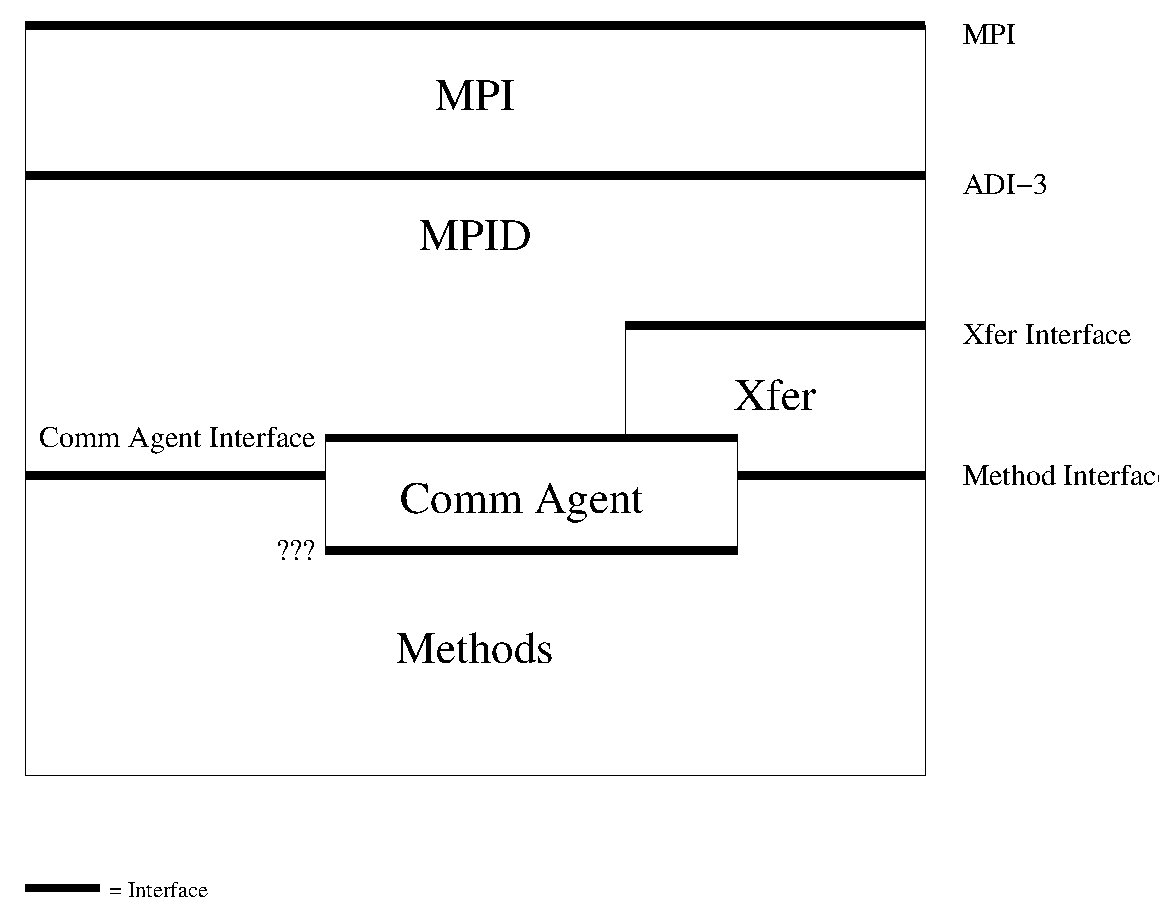
\includegraphics[height=3in]{mpich2-arch.eps}
\caption{\label{fig:arch} MPICH-2 architecture in a nutshell}
\end{center}
\end{figure}

In Figure \ref{fig:arch}, we present a diagram of the component layers
comprising MPICH2.  In this diagram, the components are respresented
by boxes and the interfaces are expressed as heavy lines between the
components.  At the top, we have the application which uses the
Message Passing Interface (MPI) as defined by the MPI Forum to
communicate data amongst its processes.  At the bottom, we have the
various communication network devices (or software interfaces) over
which the application's data might be communicated.

The MPI component layer performs a variety of tasks including
comprehensive error checking before employing the MPICH device layer
(MPID) to perform the actual communication.  The MPID layer provides
an opportunity for the hardware vendor to plug in a streamlined MPI
implementation which is highly tuned to their networking device.  It
also provides an opportunity to develop an implementation which can
coordinate communication across multiple communication networks,
chosing the best communication path between any two processes.  The
remainder of this section is dedicated to describing the architecture
of such an multi-method device.

This multi-method device, represented by the unshaded region of the
figure, simultaneously couples MPICH2 to one or more communication
networks.  The multi-method device is responsbile for choosing the
most appropriate method for communicating messages between any two
processes.  The details about how messages are communicated across any
one of these networks is managed by a method implemented specifically
for that networking device.

Third party developers may ``plug in'' additional communications
methods by implementing the interfaces defined throughout this
section.




As discussed in \ref{sec:mpid}, this layer

 At the bottom, we several network devices potentially present
several different software interfaces.  Between these two layers, we have a
series of software interfaces designed to abstract away the differences in the
various network devices while minimizing the performance lost to these
abstractions.

In this section we're mostly going to gloss over the MPI and MPID layers,
instead focusing on the Methods, Communcation Agent, and Xfer interface.

The Xfer interface is described in detail in the Collectives section.  It is
designed specifically to express pipelined operations and is tailored for use
in scatter and gather data movement operations such as those used in the the
``large sized'' van de Geijn algorithms.

The importance of the Xfer interface with respect to this section is its output
-- \emph{CARs}, or communication agent requests.  These data structures
describe actions to be performed on portions of MPI datatypes by underlying
methods.  These actions include sending and receiving of data.

The ``portions of datatypes'' are described throughout the MPICH layers as
\emph{segments}.  Hopefully segments have already been described at this
point...

% [BRT] need to elaborate on this...
% The communication agent provides two important elements to the design
% of the multi-method device.  First, it defines communication agent
% requests which abstractly convey actions to be performed by the
% communication methods.  Second, it provides a progress engine that
% manages CPU (and memory?) resources to insure that the methods cooperate.

In a common case, the communication agent is passed sets of CARs by the Xfer
interface.  These CARs are of two general types.  Send CARs are associated
immediately with the virtual connection (VC) on which they will be sent
(presumably VCs have been previously described as well).  Recv CARs are
organized in a separate set of data structures in order to facilitate easy
handling of wildcard source.  These data structures will be further described
later in this section.

Processing of these CARs is handled by what we call \emph{methods}.  These
methods are implementations of a common interface on top of a specific type of
network hardware (or really a specific network interface, such as VIA or TCP).
The bulk of the send/receive processing code exists in the method
implementations, and as such a large portion of this section will detail a
sample implementation of a method (?).

This diagram now shows the method to method interface, but we still
need to talk about it...

%------------------------------------------------------------------------------

\subsection{Proposed Nomenclature Change}

% include ca-nomenclature.eps here
\begin{figure}
\begin{center}
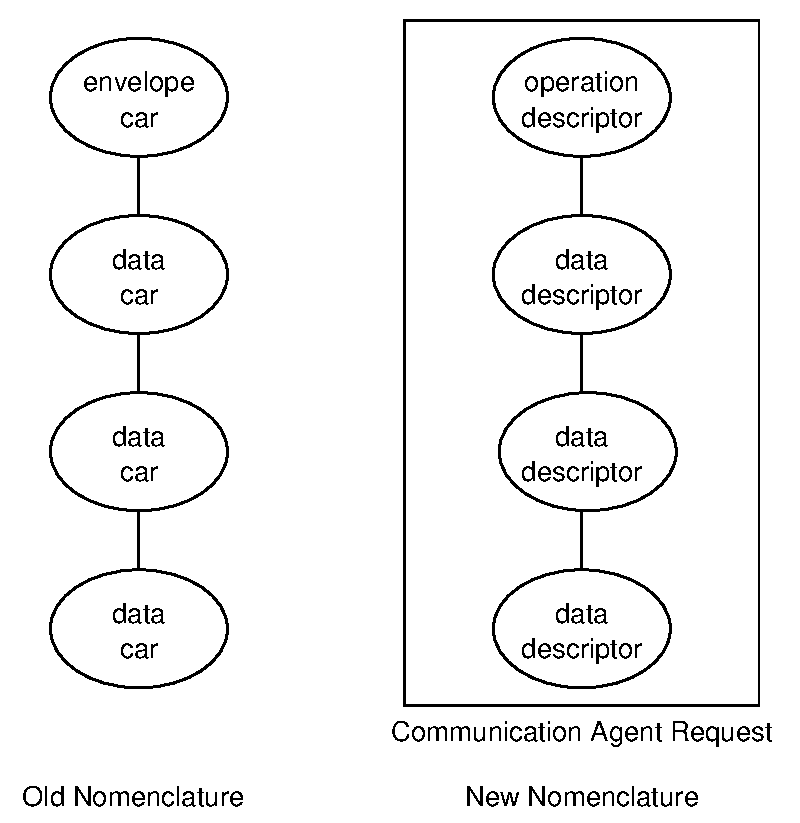
\includegraphics[height=3in]{ca-nomenclature.eps}
\caption{\label{fig:ca-nomenclature} Old and new CA nomenclature}
\end{center}
\end{figure}


Brian and I are suggesting a nomenclature change within the communication
agent.  We feel that the terms used for components previously are somewhat
misleading as things stand today.  Figure \ref{fig:ca-nomenclature} outlines
this change.  In summary:
\begin{itemize}
\item envelope cars will now be known as operation descriptors
\item data cars will now be known as data descriptors
\item the whole collection of what used to be ``cars'' (what are now
  descriptors) will be denoted as a single communication agent request (CAR).
  this entity as a whole had no single name previously.
\end{itemize}

%------------------------------------------------------------------------------

\subsection{Virtual Connections}

\begin{figure}
\begin{center}
\includegraphics[height=8in]{vc-sm.eps}
\caption{\label{fig:vc-sm} Virtual connection state machine}
\end{center}
\end{figure}

% Talk about binding, the special unbound function table, need for locks to
% avoid races when changing function table, etc.

In MPI, the application expresses the desire to communicate with particular
remote process by specifying a communicator and a rank.  The MPI implementation
is responsible for mapping these (communicator, rank) pairs to some underlying
set of network resources and performing the communication using those
resources.  To minimize startup time and avoid unnecessary resource
consumption, it is desirable for the multi-method implementation to defer
binding to specific network resoures until those resources are needed.  To
faciliate late binding, we introduce a virtual connection (VC).

A virtual connection is an object representing an abstract connection between
two processes.  Initially, the programming interfaces presented by the VC are
bound to a set of ``unbound'' functions.  These functions are responsible for
selecting the communication method to be used by this VC, rebinding the
interfaces to the functions provided by that method, and establishing a
connection using this newly bound method..

Obviously, allowing function pointer tables to change in the middle of a
running program presents a problem when running in a threaded environment.  For
that reason, is necessary to ensure that only one thread initiates the
rebinding process.  All other threads attempting to perform operation on the
same VC must either block or log the requested actions until such time as the
rebinding and connection establishment processes are complete.  Playback of
logged requests (resulting from non-blocking functions) must be handled with
care as message order within a context must be maintained.

Figure \ref{fig:vc-sm} shows a simple state machine for implementing virtual
connections.  This state machine assumes a non-threaded environment and that
all requested actions will block until the connection is established.  A
textual description of the state machines follows.

\input{vc-sm.txt}

Some proposed functions in the interface for manipulating virtual connections:
\begin{description}
\item[alloc] - return pointer to new, unreferenced vc structure
\item[add\_ref] - inc refct
\item[release] - decrement refcnt and free if refct reaches 0
\end{description}

%------------------------------------------------------------------------------

\subsection{Methods}

% [BRT] define a method
A communication method is responsible for sending and receiving
messages generated by the layers above it.

% [BRT] hmmm...which should be introduced first, CARs or methods...

% [BRT] introduce the notion of a method interface to convey abstract
% messaging requests into particular method implementations

There are some key concepts which are needed before discussing the methods:
\begin{description}
\item[packet] header, data
% include both control and data packets
\item[eager send]
\item[short send]
\item[rendezvous send]
\item[flow control]
\item[stream vs. packet interfaces]
\end{description}

% [BRT] Flow control may require transforming message requests into something
% closer to what will be sent over the wire.
There are three approaches to sending data potentially used by method
implementations.  These are commonly known as \emph{short}, \emph{eager}, and
\emph{rendezvous}.  While everyone probably has a common understanding of what
these mean in general, we will apply some specific rules in this context.

A message may be sent using the short approach only if the data contained in
the message will fit within the same unit of transfer (network packet) that the
header (control information) will be sent in.  Messages marked as being sent
using the short approach will always be sent using this approach.

A message may always be sent by the rendezvous approach.  This approach implies
that handshaking will occur before any data is transferred.  This allows for
notification from the receiver that space is available.  It also implies that
an extra round trip time will be accrued.  In our sample method it is never the
case that a message marked for sending via rendezvous will be instead sent
eagerly.

% we introduce this concept of converting here before we even talk about 
% what it means...
% TODO: FIX THIS SOMEHOW

A message may be sent using the eager approach if it is unnecessary to
handshake either due to the size of the message (it is sufficiently small) or
because the sender is guaranteeing that buffer space is available on the
receiver via some external means (e.g. ready send).  In our sample method it is
possible that a message marked to be sent eagerly will instead be sent using
the rendezvous approach.  This would be in reaction to knowledge within the
method of the status of buffers on the receiver side (i.e. the method detects
that the receiver is low on buffers).  Note, such as conversion would never be
applied to a ready send where the user buffer is guaranteed to already be known
by the receiver.

\subsection{Interfaces}

We need a buffer management interface.  This includes allocating buffers for
longer periods of time, as in persistent operations, and the allocating of
buffers during CAR processing.  Adding to the complexity of this is the need
for buffers which are usable by multiple methods.

For persistent operations, avoidance of pinning is a big win.  So if we can
send/recv from the user's buffer, then we would like to pin it once and keep
some information around (in the request?) that lets us keep up with this.  Thus
the MPID implementation will need to be able to get at the method buffer
functions.  In the case where we need to pack, we will still want to go ahead
and allocate and retain buffers in order to minimize allocation costs.

We need a request management interface.  We must be able to add requests to the
right collections, match these requests, wait on requests, and allocate and
free requests.

There will be a list of function pointers associated with the VC.  These
pointers resolve to method-specific functions and correspond to the interface
between the MPID and the method layers.

\subsection{CARs, dependencies, and all that}

One important bit of information which must be maintained throughout the
building of lists of descriptors is envelope information.  This information is
used initially to determine the source/destination for a message.  We put this
information into an \emph{operation descriptor} which is used to organize data
descriptors.

We might want to cache information such as the datatype map and/or size of the
message stored in this entity as well, although we can always derive it this
information (as long as processing hasn't started).

\subsection{Posting Operations}

% NOMENCLATURE IS CORRECT IN THIS SUBSUBSECTION

Ok, so let's assume that we have built a CAR to send, which is a string of two
descriptors.  At the head of this string is an envelope CAR with the envelope
information.  Following this is a single data CAR corresponding to a send.

This string of descriptors makes up an MPI send operation.

The operation descriptor (OD) contains comm, dest, tag, and context.  We might
eventually want the VC in there.  The context, dest, and tag must be sent
across the wire in order for the recv on the other side to match, while the
comm and dest are needed locally in order to match this CAR to the correct
VC.

The OD must also have a message type field; this is described later in this
section.

% In the more general case, we might think of this as an \emph{operation
%   descriptor car}.  It will hold info necessary for whatever
% operations...including puts and gets.

The data descriptor contains segment information.  So far that is all that is
needed.

How do we post this?  Options:
\begin{itemize}
\item vc.post\_send() -- implies that the send and receive post operations would
  be very dissimilar
\item mpid\_ca\_post\_send() -- this is more generic and could be made to look
  very symmetrical wrt the receive post operation.
\end{itemize}

The second option leads us to define the VC structures well and allow the CA
coponents to manipulate them.  Furthermore, we would still have to have some
mechanism for notifying the underlying VC code that a new request had been
posted.  This is necessary in order to guarantee that the state machine knows
that it can make progress -- essentially we're notifying it of a post event.

The first option allows us to get straight to the right function w/out going
through some intermediate code at the cost of having to discover the VC at this
higher level.  We are leaning towards this approach, and we will proceed with
this one.

We've bypassed any notion of a CA at this point, instead sending the CAR
directly to the method.

\begin{verbatim}
vc::post_send(car)
\end{verbatim}

We could have handled this specific case more quickly if we didn't have to allocate the operation and data cars just to send them to the method like this.  BUT we need them in order to hold their places in the queues (bad word) in the case where things aren't all ready to go.  Is it worth having the method allocate these only if needed in order to optimize for the simple send case?

\begin{verbatim}
vc::post_simple_send(comm, context, dest, tag, counter_pointer, segment)
\end{verbatim}
There are many cases where the VC isn't currently doing anything and the method
is simple enough that one could imagine that one wouldn't need to build the
cars a fair amount of the time.

Another option would be:
\begin{verbatim}
vc::post_send_cars(nr_cars, car_array)
\end{verbatim}
This would be helpful in the RMA case where multiple puts, for example, could
then be posted with a single call.

Proposal:
\begin{verbatim}
vc::post_send_msg(comm, dest, tag, counter_pointer, segment, type, flags)
vc::post_send_cars(nr_cars, send_car_array)
\end{verbatim}
Two functions, one to send a point to point message without necessarily
imposing the overhead of building the CAR, and another to submit one or more
pre-build cars.  The latter is useful for aggregating multiple RMA operations,
but it would also be used to post a CAR which is made up of more than one data
descriptor (nr\_cars = 1 in this case).

The type field is used to differentiate between specific send scenarios, such
as the special case of the synchronous send.  These types may be translated
once inside the method layer and this field could then used to maintain the
mechanism by which data is being moved: via short, eager, or rendezvous
messages (don't like this term).

There are two categories of types.  The first of these are types which may be
passed from above the method layer through the post functions.  The types of
interest currently are:
\begin{itemize}
\item normal send - the standard send case; nothing special; we might cut it
\item synchronous send - we'll want to use rendezvous sends in most methods for
  this
\item ready send - we need to send notification of this type of send along in
  the message so that the other end can detect the erroneous condition of an
  unexpected ready message.
\end{itemize}

The second category of types are ones which might optionally be used by the
method implementation as part of internal processing.  We will cover one
example of such a set of types in order to clarify our prototype method state
machine.

Additionally there are optional flags which may be passed in to these calls:
\begin{itemize}
\item direct access - the segment buffer is directly usable by this method (is
  this reasonable?)
\end{itemize}

The direct access flag is of use in the persistent operations.  Note that I
(Rob) suggest we punt on trying to support direct access in the wildcard
receive case.

It is acceptable for the method to augment this list of flags with additional
flags used within the method during processing.

We're going to skip post\_send\_msg() as it is really just an optimization, and
we're going to instead cover post\_send\_cars() and how this is handled.

We still have our simple one-data-descriptor CAR.

Let's assume that there is nothing in the VC send queue at the time this is
posted.

\begin{verbatim}
post_send_cars(nr, car_array)
{
    // We also need to handle Rsend and Ssend.  Rsend requires an extra bit in
    // the message meta-data informing the receiver that this is a ready send.
    // Ssend can be implemented by forcing a rendezvous exchange, although this
    // may not be the most efficient mechanism.

    foreach car
        compute message size from DDs and store it in the OD
        switch(new_type = type_of_message(size, OD.type))
        case Eager:
            if OD.type == ready send
                flags |= dont_convert
                flags |= send_ready_bit
        case Short:
            if OD.type == ready send
                flags |= send_ready_bit
        case Rndv:
            // this one is a little wacky -- dunno what goes here yet
            // this could be converted to a rndv-rts and then converted to
            // a rndv-data, or just converted to rndv-data and a new CAR
            // could be created to submit the rndv-rts
        OD.type = new_type
        add car to send queue
    if send queue was empty before we started
        // we missed a little optimization by not triggering on first enqueue.
        trigger a [CAR Available] event
    update any method status information to indicate outstanding requests
    call poll/make progress function (could be a CA function or maybe a method 
      one)
}
\end{verbatim}

Contents of an operation descriptor:
\begin{itemize}
\item message type ([normal|synchronous|ready])
\item comm/context
\item destination rank
\item tag
\item pointer to counter
\end{itemize}

Contents of a data descriptor:
\begin{itemize}
\item flags (direct access, ?)
\item segment
\end{itemize}

% \subsection{Recv CAR Processing}

How do we post receives?  Options:
\begin{itemize}
\item vc.post\_recv() -- gets us a symmetric interface in the vc
\item mpid\_ca\_post\_recv() -- more generic, symmetric at the CA level
\end{itemize}

The interesting thing about the first option is the wildcard case.  There is no
``real'' vc on which to call a function.  So we create a wildcard VC to handle
this.  Then we can do wildcard sends too :).  This creates a situation where
method implementors can freely implement new receive post functions as well,
which may be of only limited value.

The second option is arguably more straight-forward, but it adds an additional
call to the path and isn't as cool as a wildcard VC :).

%
% TODO: TALK ABOUT THIS MORE
%
We would probably implement a single helper function for posting receives that
is used by all the methods to do most of the right stuff.  Of importance here
is the fact that notification does need to occur to specific methods, say in
the case where an unexpected receive (in progress) is matched to this posted
receive.

I (Rob) feel that the inclusion of the send and receive post operations in the
VC function table is more aesthetically pleasing -- it just seems like the
right thing.  I think all these CAR-manipulation calls should be there...

%
% XFER INTERFACE
%
\subsection{Xfer Interface}


\subsection{CAR Management}

Here we're talking about MPID requests.

Send requests get queued on VCs in the order in which they are submitted.  This
is necessary for meeting the MPI ordering rules.

Receive requests are posted through a common interface:
\begin{verbatim}
THIS IS THE INTERFACE
\end{verbatim}
This interface is used to hide the implementation of the matching
functionality, because we don't think we really know how we want this to be
implemented yet.  We have considered putting all receive requests on a single
list, using the Rajeev per-method system, and other options (e.g. a per-VC
posted list with global wildcard and unexpected lists and a counter to
maintain ordering).  Comments?

It might make sense to make this common interface one more function in the VC
function table.  This would be nice from an organizational view, and it leaves
us the option of replacing the function on a by-method basis if we wanted to
later (say, if we wanted to implement per-method non-wildcard-capable functions
just for fun).

We are currently thinking that we want to have a separate post send and post
receive, because we think that these are going to quite different places.  In
the xfer case we will have a number of requests/operations which will need to
be posted at once; it might make sense to have a function that can handle all
these in a single call, or perhaps a pair, one for handling all the sends and
another for all the receives.

In any case, all locking on the recv request data structures will be handled
inside the post function.

We feel that there will be some method-specific information which will make its
way into the request structure.  We would like to allocate all the memory for the request structure as a unit.  There are two obvious methods for doing this:
\begin{itemize}
\item a per-method request allocation function
\item a single request allocation function which uses knowledge of the
  method-specific data structure sizes (perhaps acquires at initialization
  time)
\end{itemize}
The second option allows for cross-method use of the same requests, which will
help with memory utilization and might turn out to be mandatory for forwarding
(?).

This same argument holds for CARs.

Requests will hold a counter which will be used to implement the MPI wait and
test functions.  This counter will be set to the number of CARs associated with
the request before its associated CARs are queued for service.  As CARs are
completed, the counter is decremented.  Once the counter reaches 0, the request
is complete with respect to all underlying data transfer.  This counter can be
checked by the MPI wait and test function implementations (or MPID?).

Proposed change: let's have a counter, but let's decrement it based on
completion of a string rather than each individual component of the string.
One way to do this would be to have a special type of descriptor at the end (a
counter descriptor) which does the decrement.  Alternatively we could keep
pointers back to the OD/envelope car and don't free it immediately.

%
% BEGIN OLD AGENT.TXT TEXT
%
- there is also a global "unexpected receive" queue in which incoming sends
  which do not match are placed.

- there is also a wildcard queue, possibly one per method.  we will devise some
  mechanism for avoiding locking this queue each time we receive an incoming
  send.  some alternatives are: one wc queue per method, an is-empty flag for
  the wildcard queue (which must be capable of being atomically read or written
  without a lock).  WE WILL HAVE ONE WILDCARD QUEUE ONLY.

- this will let us do per-communicator "no wildcard" attributes if we like as
  well :).

- a receive call from above matches the unexpected queue and then inserts
  itself into the wildcard of vc-specific queue

- an incoming message from a remote system matches the wildcard queue or the
  vc-specific receive queue.  to maintain MPI ordering semantics, we must keep
  a counter.  this counter's value is stored in each CAR.  it is incremented
  only on enqueue into the wildcard queue (new value used by wildcard CAR), and
  ties go to the wildcard receive.  

- we will have to handle rollover in some reasonable way...how do we want to do
  that? i propose some very high overhead mad search through things in order
  to teach these evil wildcard users a lesson!

end result: we have rewarded the case where receives are posted first with only
per-vc locks.  in the case of wildcard receives we have a counter increment and
a second queue to check.  in the case of unmatched incoming messages we have a
single queue which might be a source of some contention.

this is a more memory-intensive approach than the original prototype, but it
should allow for higher performance and parallelism across VCs that share a
common method at least in the well-behaved case of pre-posted, known-source
receives (which is the approach we should reward :)).

- we decided to use a single unexpected queue since having multiple unexpected
  queues requires timestamp to order the messages.  the timestamp counter is a
  point of global contention, just like the global unexpect queue.

- this same argument can be applied to the posted queue case, but allowing for
  multiple queues here creates a much nicer search situation for the case where
  people prepost their receives.  is this worth the cost of the counter
  manipulation?

  for the non-threaded, non-shmem case we think this will be a win.  for the
  case of threads or shmem, we are unsure if the lock overhead of the queues
  and counter increment will result in a loss.

  SINCE WE CAN'T COME TO A REAL CONSENSUS, WE WILL HIDE THIS BEHIND AN API.
  then we can play with the implementation ad nauseum, just as we have with
  this conversation :).

ASIDE:
  rusty and rajeev broke queues into a queue per method, with each method
  implementing its own queue code.  they then had a separate wildcard queue,
  and wildcards were ALSO posted in each method queue.

%
% END OF OLD AGENT.TXT TEXT
%


%
% PROCESSING CARS
%
\subsection{Processing CARs}

blah

%
% SEND STATE MACHINE
%
\subsubsection{Send State Machine Diagram}

Key components:
\begin{description}
\item[event]
\item[action]
\item[state]
\end{description}

Figure \ref{fig:send-sm} shows a sample method send state machine.

\begin{figure}[h]
\begin{center}
\includegraphics[height=8in]{send-sm.eps}
\caption{\label{fig:send-sm} Send state machine}
\end{center}
\end{figure}

\subsubsection{Send State Machine Description}
\input{send-sm.txt}

%
% RECV STATE MACHINE
%
\subsubsection{Recv State Machine}

%
% RENDEZVOUS AND LIBAS
%
\subsubsection{Rendezvous Messages and LIBAs}

% TODO: clean this up -- the wording sucks...
The processesing of rendezvous clear-to-send and data messages requires the
ability to locate the CARs that are the target of those messages.  To
facilitate this, we introduce the notion of a locally interpretted byte array
or a LIBA.  In our sample method, LIBAs are used to pass a reference to a
operation descriptor as part of the message control information.  As is implied
by ``local'', the contents of a LIBA are only meaningful to the process that
created it.  This allows us to quickly find matching descriptors on reception
of handshaking packets (?) which are passed during the rendezvous setup.

The following outlines the anticipated exchange needed to send a message using
the rendezvous technique in MPICH-2.
\begin{itemize}
\item The sender sends a request-to-send (RTS) message which contains the
  envelope information a LIBA referring to the send CAR.
\item When the receiver receives the RTS message, it performs an incoming find
  or allocate CAR operation.
\item If a CAR matching the envelope has already been posted, the receiver
  immediate send a clear-to-send (CTS) message back to the sender.  This
  message contains the sender's LIBA as well as a LIBA referring to the
  matching receive CAR.  Otherwise the sender's LIBA is recorded in the
  unexpected CAR and the CTS is sent when the message is posted by the
  application.
\item When the sender receives the CTS message, it may begin transmitting the
  message data.  It uses the sender's LIBA located in the message to find the
  send CAR.  Once the send CAR is located, a rendezvous data message is sent
  containing the receiver's LIBA and the message data.
\item The receiver uses the LIBA in the rendezvous data message to locate the
  associated receive request and determine where to store the incoming data.
\end{itemize}



\subsection{Cleanup}

\subsubsection{Signalling Send CAR Completion}

A send CAR is considered complete when all data in the user buffer has been
sent or buffered.  Once a CAR has completed, it is necessary to signal the
requestor of this completion.  This is accomplished by atomically decrementing
a counter provided by the requestor -- this is how the MPID layer knows
progress has been made on some portion of an MPI request.

There are two factors at work here.  First it is necessary that the user
buffer not be modified until all the data in it has been processed (either via
copy or sending).  Second we want to notify the upper layer as quickly as
possible that these operations have been performed so that the upper layers may
return control of buffers to the application and allow MPI wait operations to
complete.

Determining when the buffer is no longer needed depends on
whether the data is being sent directly from the user buffer (direct access),
copied into a series of packet buffers, or some combination thereof.

There are three cases to consider with respect to processing of data:
\begin{itemize}
\item all user data is buffered by the method
\item all user data is accessed directly
\item some user data is buffered, while other portions are accessed directly
\end{itemize}

In the first case, the user buffers are available for re-use immediately after
all the sends are posted.  In this case the send state machine can be
responsible for signalling CAR completion.

It is not desirable in the second case for the send state machine to wait for
the sends to complete so that it can signal CAR completion, as we would like
for it to move on to the next CAR.  Thus we must use a separate mechanism for
signalling completion in the direct access case.  We must have a mechanism to
associate the CAR with the last posted packet descriptor, allowing the packet
reclamation code to perform the signalling when the packet descriptor is
reclaimed.  Ideally this association would be made by placing a reference to
the CAR in the network packet descriptor.

In the third case, we must not signal completion until the data to be buffered
has been copied into packet buffers and the direct access data has been sent.
This case can be handled in the same manner as the second (direct access only)
case; however, we lose the opportunity to perhaps signal completion sooner if
we use this approach.  In particular, if there is a large amount of buffered
data at the end of the transfer, then completion could be signalled as soon as
this data is buffered and posted.

In order to accomplish this more aggressive signalling, we need to detect both
of the following conditions have been met:
\begin{itemize}
\item all of the data to be buffer has been copied into packet buffers, and
\item all of the direct access data has been sent.
\end{itemize}
This detection is complicated by the fact that the first condition will be met
in the state machine, while the second condition will be met in the buffer
reclamation system, both of which may be concurrently active.

On approach is to add an outstanding activities counter which is intialized to
a value of two (2), indicating that neither condition has been met.  Then, the
following code would be executed when each of the individual conditions is met.
The send state machine would execute this code when all user data has been
buffered.  The reclamation mechanism would execute this code when all directly
accessed data associated with this CAR has been successfully sent.
\begin{verbatim}
lock OD.mutex
    decrement CAR outstanding activities counter
    if the outstanding activities counter has reached zero
        signal completion (decrement completion counter)
unlock OD.mutex
\end{verbatim}

%
% RECLAMATION
%
\subsubsection{CAR and Method Buffer Reclamation}

talk about buffer reclamation and CAR reclamation here (not necesarily in that
order).

direct access (user buffer)
\begin{itemize}
\item no buffer reclamation
\item CAR is not complete until send from the user buffer is complete
\end{itemize}

packet buffers
\begin{itemize}
\item must do buffer reclamation
\item CAR is complete as soon as last of data is copied into a packet buffer
\end{itemize}

%
% COMM AGENT
%
\subsection{Communication Agent (CA) and Making Progress}

There are some key concepts which are needed before discussing the CA.  They
might be covered somewhere else, but in case they aren't:
\begin{description}
\item[virtual connection (VC)] -- an object which is an abstraction of a point
  to point connection which allows for late binding to a communication method
  (and thus a physical connection) and provides a common interface to
  particular method implementations
\item[communication agent request (CAR)] -- a low level description of an
  operation to be performed by a method and the data involved in the operation
  (are these really cars any more?  they don't really go through an agent...or
  do they in the rma or other cases?)
\item[MPI/MPID request] -- a high level structure used primarily as a handle on
  which to track the status of asynchronous operations.
\item[buffer] -- we refer to two types of buffers: user (or MPI) buffers and
  method (or packet) buffers.  MPI buffers are regions of user address space
  which are passed to MPI calls.  method buffers are regions of memory
  allocated for use by the underlying methods in the MPICH-2 implementation for
  performing data movement operations.
\item[segment] -- a segment is a portion of an MPI buffer.  this is described
  by a datatype, a count, an address, and first and last offsets into the
  buffer.
\item[MPI envelope] an MPI envelope consists of a context, tag, and rank (of
  source or destination, depending on operation)
\end{description}

The CA will in some (but not all) cases fill the role of polling/driving the
methods.  Specifically, some methods are perfectly capable of driving
themselves for some common operations (e.g. TCP with its own thread).  However,
in the case of a non-threaded implementation, for example, the CA will
implement the necessary functions which may be called by the MPID
implementation to ensure that progress occurs.

One important possible optimization is the use of different polling frequencies
and adaptive polling on methods.  The appropriate place to implement such an
optimization is in the CA, as there is no efficient manner in which the methods
can self-impose this type of behavior (they would individually have to read a
clock all the time or something equally inefficient).

Methods could write status information into a shared region that the CA could
use for this adaptive polling technique.  In this way we could avoid using
function calls to obtain the information.

%
% MAKING PROGRESS
%
%\subsection{Making Progress}

talk about mpid\_cond\_wait() here.


\end{document}
